\section{Nodal Analysis}
\label{sec:nodal analysis}

\subsection{Systematic procedure}
In this circuit, there are 8 nodes. Therefore, to solve the circuit we need to find N (number of nodes) -1 equations, which in this case means we must find 7 independent equations. Firstly, we must choose our ground node (node which, by convention, has voltage 0). Typically the node chosen as the ground node is the one that connects to a voltage source so we chose the node that connects the voltage source $V_{a}$ and the resistors 4 and 6. Next, we numbered the remaining nodes as shown in Figure ~\ref{fig:nodes}.

\begin{figure}[ht] \centering
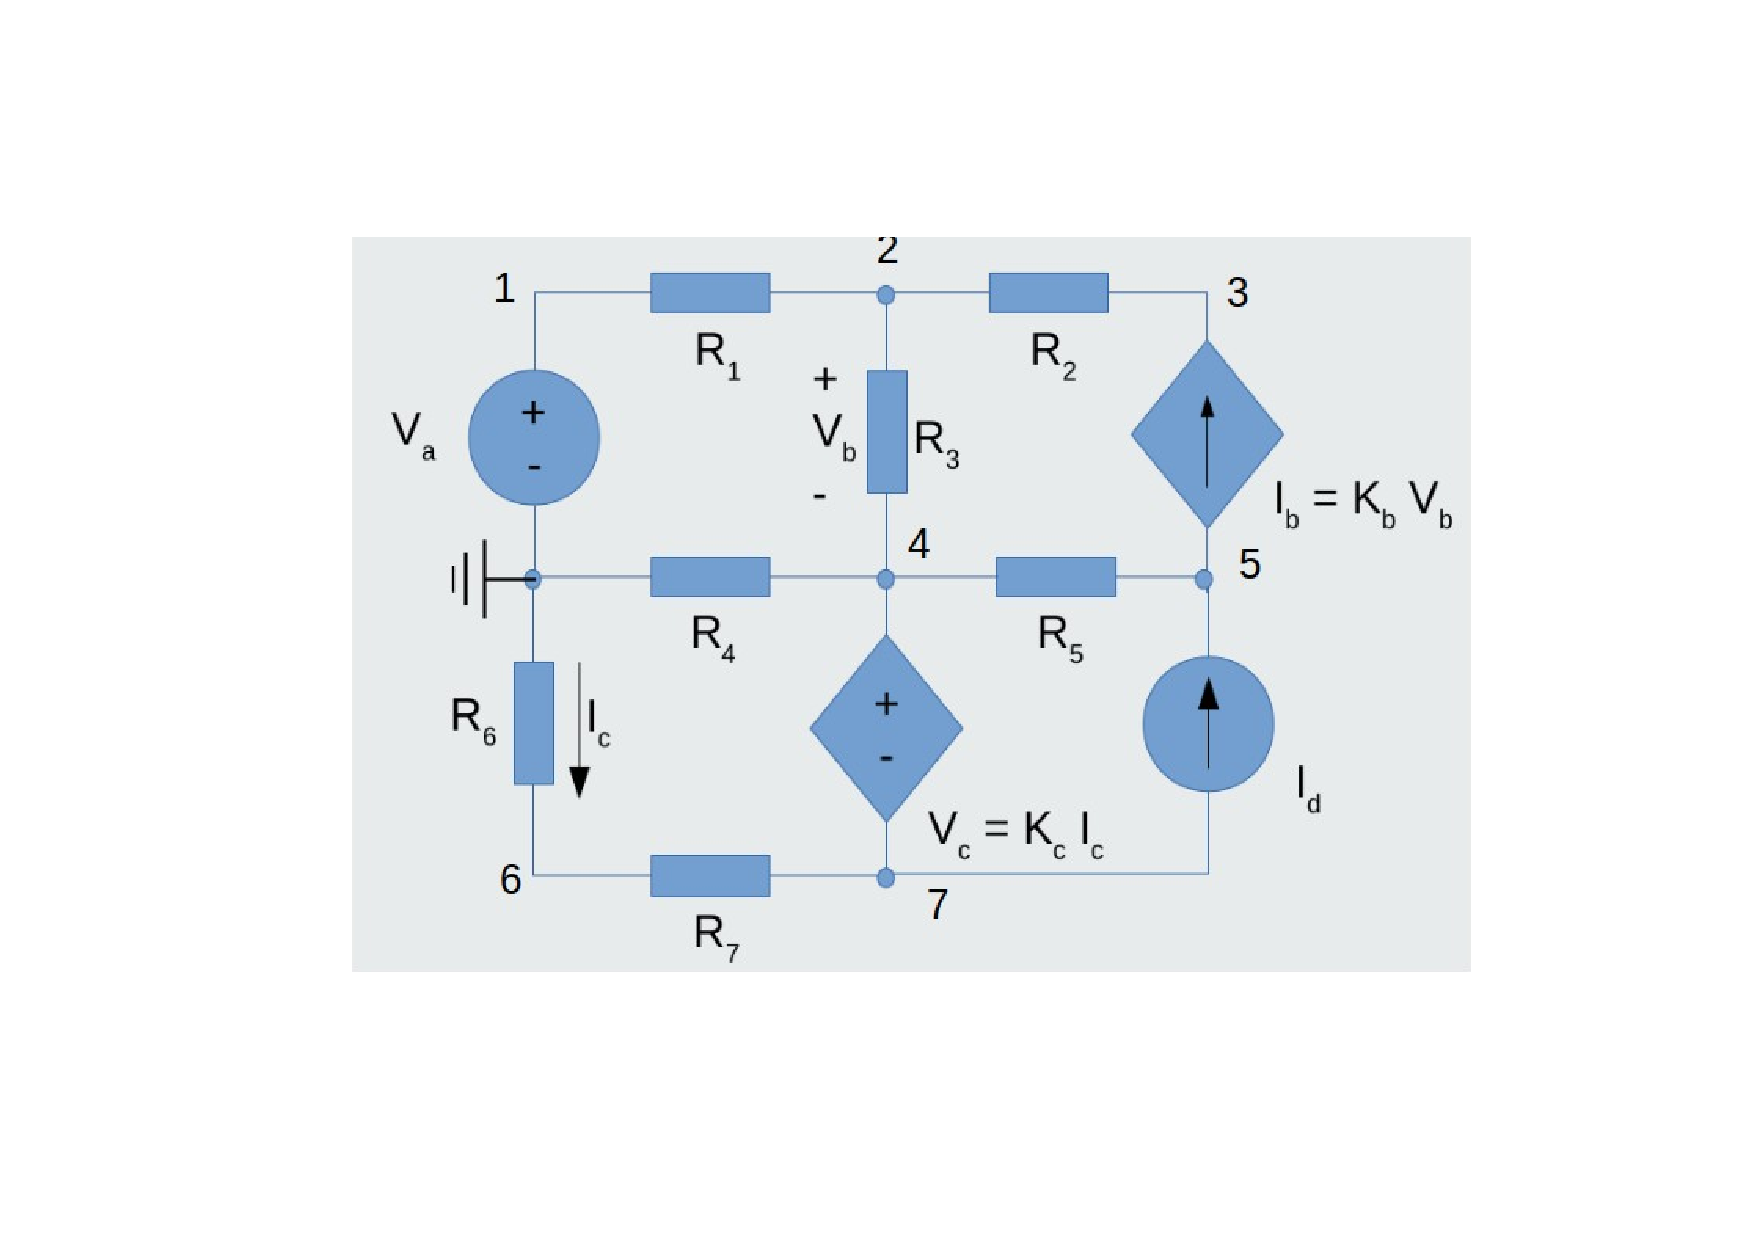
\includegraphics[width=0.8\linewidth]{circuitonodos.pdf}
\caption{Numbered nodes and ground node}
\label{fig:nodes}
\end{figure}
\subsection{Discovering the equations}
Now to discover the equations for each node we need to use Kirchhoff’s Current Law, which states that the sum of all the currents entering and leaving a node must be equal to zero. For simplicity instead of using directly the currents we will also use Ohm's Law. \\
Starting off at node 1, we will consider that current is leaving node 1 towards the voltage source and that current is entering the node from the resistor 1. That leaves us with the following equation:
\begin{equation}
     -i_{a}+\frac{V_{2}-V_{1}}{R_{1}}=0 \Leftrightarrow i_{a}=\frac{V_{2}-V_{1}}{R_{1}},
\end{equation}
where $V_{1}$ and $V_{2}$ are the voltages at nodes 1 and 2 and $i_{a}$ is the current that flows through the voltage source. \\
Moreover, we know the voltage provided by the voltage source is equal to $V_{a}$. Taking into consideration the voltage at the nodes 1 and ground we get:
\begin{equation}
    V_{a}=V_{1}-V_{GND} \Leftrightarrow V_{a}=V_{1}
\end{equation}
where $V_{GND}$ is the voltage at the ground node (by convention = 0).\\
Now looking at node 2. We consider all currents entering the node. From that we get:
\begin{equation}
  \frac{V_{1}-V_{2}}{R_{1}} +\frac{V_{3}-V_{2}}{R_{2}}+\frac{V_{4}-V_{2}}{R_{3}}=0
\end{equation}
Moving along to node 3. Here we have a current that is already named, $I_b$. We consider the current moving as is indicated by the symbol, so entering node 3 and then we also consider that current is leaving node 3 toward the resistor 2. This leaves us with:
\begin{equation}
    I_{b}-\left(\frac{V_{3}-V_{2}}{R_{2}}\right)=0 \Leftrightarrow I_{b}=\frac{V_{3}-V_{2}}{R_{2}}
\end{equation}
Next on the list is node 4. Here we consider that current is leaving the node towards resistor 5 and the current dependant voltage source $V_{c}$ and entering the node from resistors 3 and 4. The KCL equation becomes:
\begin{equation}
    -i_{c}-\left(\frac{V_{4}-V_{5}}{R_{5}}\right)+\frac{V_{2}-V_{4}}{R_{3}}+\frac{V_{GND}-V_{4}}{R_{4}}=0 \Leftrightarrow i_{c}+\frac{V_{4}-V_{5}}{R_{5}}+\frac{V_{4}-V_{2}}{R_{3}}+\frac{V_{4}}{R_{4}}=0 
\end{equation}
where $i_c$ is the current through the current dependant voltage source.\\
From nodes 2, 3 and 4 we can also extract one more equation. Because of the voltage dependant current source and the resistor 3 we know 2 things about $V_{b}$:
\[V_{b}=V_{2}-V_{4} \hspace{5mm} V_{b}=\frac{I_{b}}{K_{b}} \]
Using equation (4) we can further develop this relation between the two equations.
\begin{equation}
    V_{b}=\frac{I_{b}}{K_{b}} \Leftrightarrow V_{b}=\frac{V_{3}-V_{2}}{R_{2} K_{b}} \Leftrightarrow V_{2}-V_{4}=\frac{V_{3}-V_{2}}{R_{2} K_{b}} \Leftrightarrow V_{2}-V_{4}+\frac{V_{2}-V_{3}}{R_{2} K_{b}}=0
\end{equation}
Now onto node 5. We again use the already named voltage dependant current, $I_{b}$ (that is defined in equation 4) and current source $I_{d}$. We define the current direction in accordance with their symbols ($I_{b}$ is leaving the node and $I_{d}$ is entering). We also have a resistor, resistor 5, and we assume current is leaving the resistor and entering the node. 
\begin{equation}
    -I_{b}+I_{d}+\frac{V_{4}-V_{5}}{R_{5}}=0 \Leftrightarrow 
    \frac{V_{3}-V_{2}}{R_{2}}+\frac{V_{5}-V_{4}}{R_{5}}=I_{d}
\end{equation}
The next node is node 6. Here we have a named current entering the node, from resistor 6 called $I_{c}$, and we assume that current is leaving the node towards resistor 7. 
\begin{equation}
    I_{c}-\left(\frac{V_{6}-V_{7}}{R_{7}}\right)=0 \Leftrightarrow 
    \frac{V_{6}-V_{7}}{R_{7}}=I_{c} 
\end{equation}
We also know that
\begin{equation}
   I_{c}=\frac{V_{GND}-V_{6}}{R_{6}}=\frac{-V_{6}}{R_{6}}  
\end{equation}

Combining this with equation (8) we get:
\begin{equation}
    \frac{V_{7}-V_{6}}{R_{7}}-\frac{V_{6}}{R_{6}}=0 
\end{equation}
    The final node is node 7. Here we again come across named current $I_{d}$ and current dependant voltage source $V_{c}$. Current $I_{d}$ is leaving the node and current is entering from the current dependant voltage source and resistor 7. The KCL equation becomes:
    \begin{equation}
     i_{c}+ \frac{V_{6}-V_{7}}{R_{7}}-I_{d}=0 \Leftrightarrow
     i_c+ \frac{V_{6}-V_{7}}{R_{7}}=I_{d}
    \end{equation}
    Since we have common terms we can combine equations (5) and (11) and get:
    \begin{equation}
I_{d}+\frac{V_{7}-V_{6}}{R_{7}}+\frac{V_{4}-V_{5}}{R_{5}}+\frac{V_{4}-V_{2}}{R_{3}}+\frac{V_{4}}{R_{4}}=0 
    \end{equation}
    At this point, we have 7 variables (the voltages at the 7 nodes) and only 6 equations. However, we know that:
    \[ V_c= V_4-V_7 \hspace{5mm} V_c=K_c I_c\]
    Combining this fact with equation (9) we get:
    \begin{equation}
        V_4 -V_7+\frac{K_c V_6}{R_6}=0
    \end{equation}
The next step is to solve the system of equations resulting from equatios 2, 3, 6, 7, 10, 12 and 13 for the node voltages:

    \begin{equation}
\left(\begin{array}{ccccccc} 
1 & 0 & 0 & 0 & 0 & 0 & 0\\
\frac{1}{R_1} & -\frac{1}{R_1}-\frac{1}{R_2} -\frac{1}{R_3} & \frac{1}{R_2} & \frac{1}{R_3}& 0 & 0 & 0 \\
0 & 1+\frac{1}{R_2 K_b} & -\frac{1}{R_2 K_b} & -1 & 0 & 0 & 0 \\
0 & -\frac{1}{R_3} & 0 & \frac{1}{R_3} +\frac{1}{R_4}+\frac{1}{R_5} & -\frac{1}{R_5} & -\frac{1}{R_7} & \frac{1}{R_7} \\
0 & -\frac{1}{R_2} & \frac{1}{R_2} & -\frac{1}{R_5} & \frac{1}{R_5} & 0 & 0 \\
0 & 0 & 0 & 0 & 0 & -\frac{1}{R_6}-\frac{1}{R_7} & \frac{1}{R_7} \\
0 & 0 & 0 & 1 & 0 & \frac{K_c}{R_6} & -1 \\
\end{array}\right)
\left(\begin{array}{c} V_1 \\ V_2 \\ V_3 \\ V_4 \\ V_5 \\ V_6 \\ V_7 \end{array}\right) 
= \left(\begin{array}{c} V_a \\ 0 \\ 0 \\-I_d \\I_d \\ 0 \\0 \end{array}\right)
\end{equation}
